% !TEX root = msc_thesis.tex

\chapter{Future directions} \label{ch:future_directions}


\section{Multitask learning of mutation deleteriousness and energetic effects} \label{sec:multitask_learning}

%  For example,  and are much more diverse, they could contribute much information to the ELASPIC predictors. Some possible ways in which this could expand and incorporate more information into the ELASPIC training set are discussed in

In this work, we attempted to improve the generalizability of ELASPIC core and interface predictors by keeping track of their performance on mutation deleteriousness datasets throughout cross-validation and feature elimination (Figures \ref{fig:gridsearch_core}, \ref{fig:gridsearch_interface}, \ref{fig:feature_elimination_core} and \ref{fig:feature_elimination_interface}). While this approach allows us to discard predictors that overfit the training set, it does not improve the accuracy of any individual predictor.

The performance of core and interface predictors on the training sets is highly correlated with their performance on the deleteriousness datasets. We could improve the overall accuracy of the predictors by leveraging the information contained in mutation deleteriousness datasets to discover better and more informative features. Since the mutation deleteriousness datasets contain 10 to 100 times more mutations than the training sets, they may allow sequential and structural features to ``mix'' in a more general environment, and produce combined features that are less noisy and better correlated with the actual effect of mutations.

We could learn those features by first training a boosted decision tree algorithm to predict mutation deleteriousness, and then using the output of those trees as input to a logistic regression model trained to predict mutation $\Delta \Delta G$ (Figure \ref{fig:multitask_learning}). The resulting predictor should not only have better accuracy, but should also have a better ability to extrapolate than the current gradient boosted regressor algorithm, which never predicts values that are higher or lower than the maximum or minimum value observed in the training set.

\begin{figure}[!htb]
	\centering
	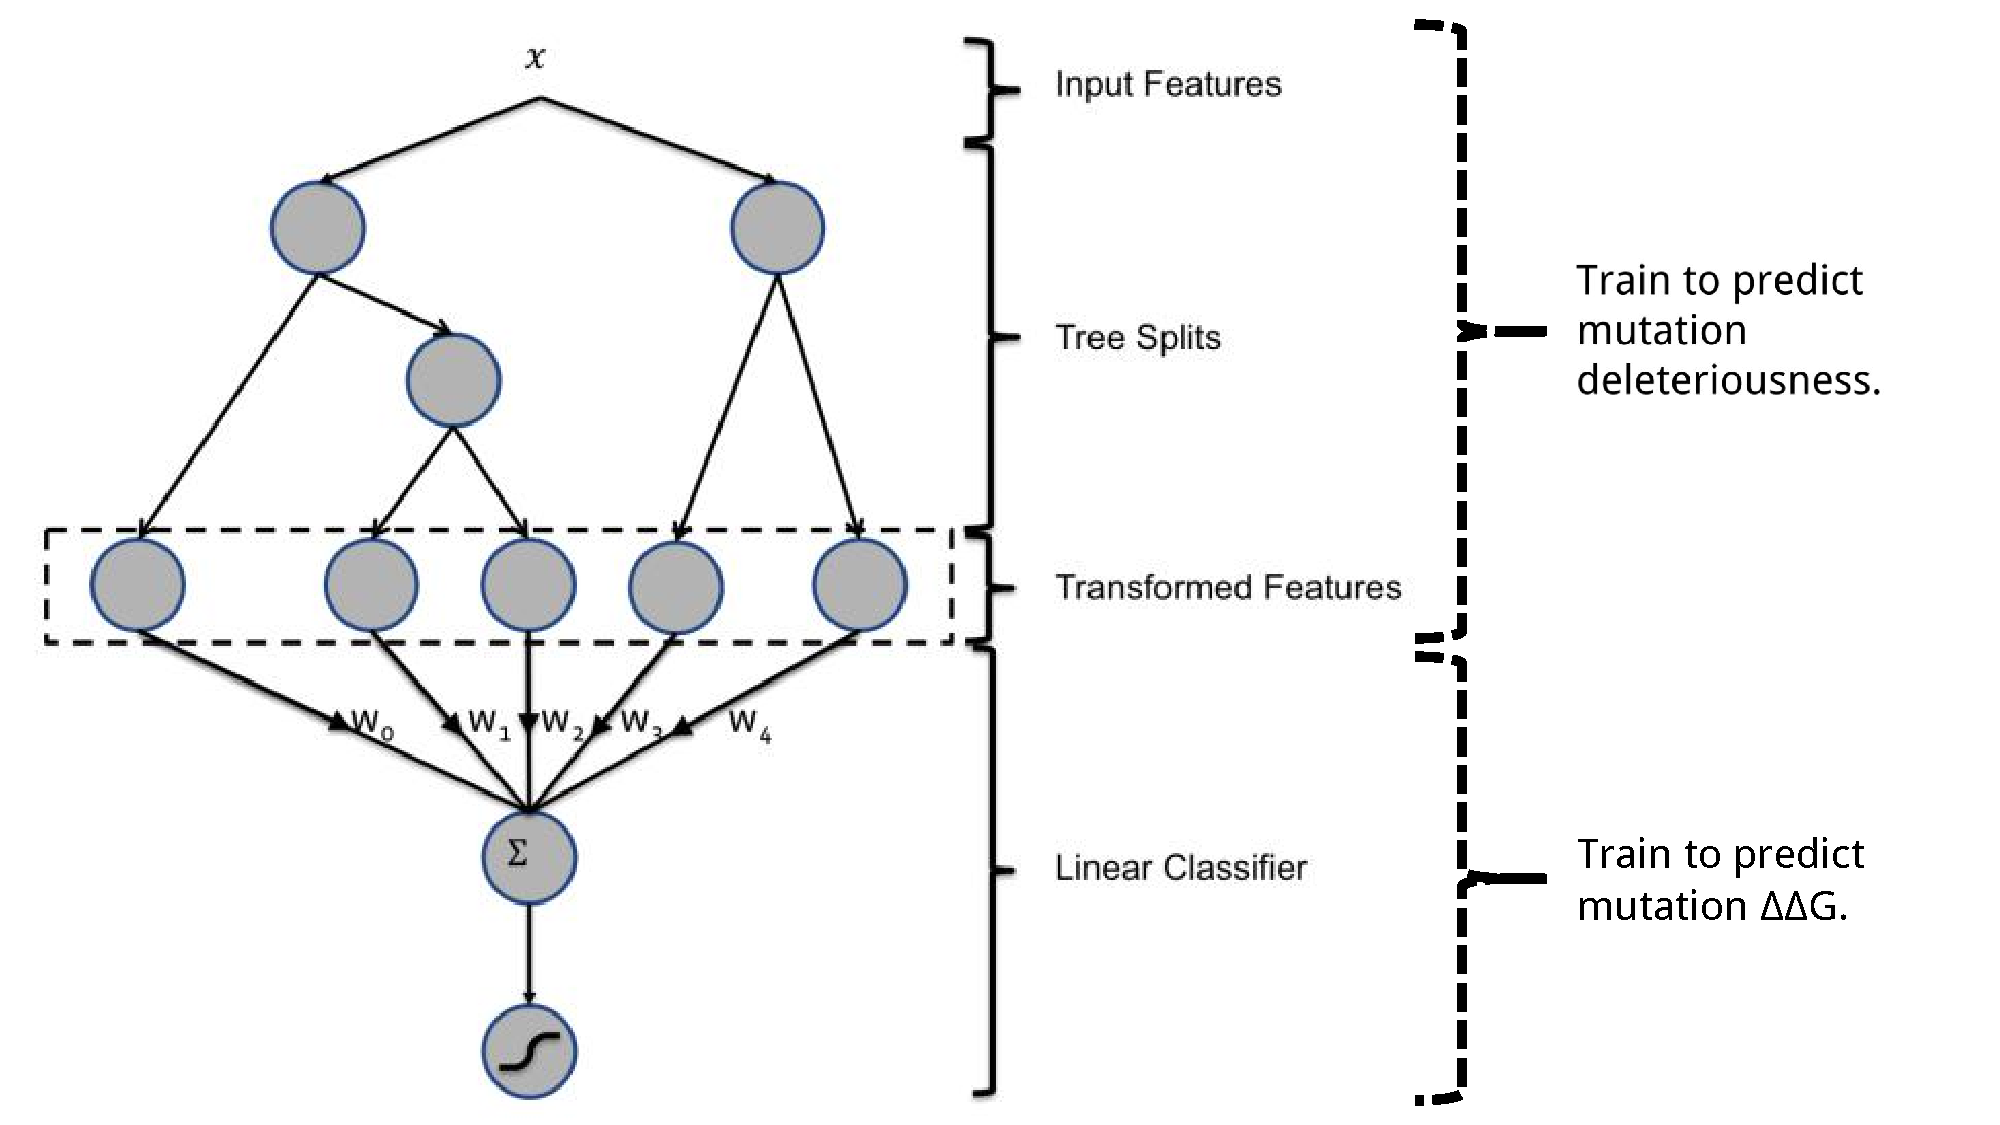
\includegraphics[width=0.8\textwidth]{static/elaspic/multitask_learning.pdf}
	\caption[Multitask learning of mutation deleteriousness and $\Delta \Delta G$.]{
		Multitask learning of mutation deleteriousness and $\Delta \Delta G$.
        The figure is adapted from He \textit{et al.} \cite{he_practical_2014}, where it is used to describe an algorithm that couples boosted decision trees and linear regression to predict add click-trough rate. Boosted decision trees are used to learn a feature ``manifold'' that is provided as input to the linear classifier, which in turn makes the final predictions. \\
        We propose to use a similar design, but train boosted decision trees to predict mutation deleteriousness, and fit a linear regressor to predict mutation $\Delta \Delta G$. We anticipate that the large training set of benign and deleterious mutations would allow the boosted decision tree algorithm to learn useful and generalizable features.
	}
	\label{fig:multitask_learning}
\end{figure}


\clearpage
\section{Adding support for multi-residue mutations} \label{sec:more_data}

Around one third of experimentally determined $\Delta \Delta G$ values in the Protherm and Skempi databases correspond to changes in multiple amino acids. While ELASPIC currently supports only single residue mutations, we could leverage the information contained in multi-residue mutations by treating them as sets of single residue mutations with the experimental $\Delta \Delta G$ approximated using the following strategy:

% \vspace{-\topsep}
\begin{enumerate}
	\itemsep0em
    \item Use ELASPIC to introduce each constituent single residue mutation, one at a time.
    \item Keep the $\Delta \Delta G$ for the single residue mutation with the most stabilizing effect.
    \item Repeat steps 1 and 2 for the remaining mutations, using, as the starting point, the structure containing the mutations selected in the previous steps.
		\item Normalize the predicted $\Delta \Delta G$ of each single residue mutation in order to make the total equal to the experimental $\Delta \Delta G$ of the multi-residue mutation.
		\item Add single residue mutations with the corresponding normalized $\Delta \Delta G$ values to the ELASPIC training set, retrain the classifiers, and repeat steps 1 to 5 until normalized $\Delta \Delta G$ values do not change between iterations.
\end{enumerate}

If ELASPIC is able to predict the $\Delta \Delta G$ of multi-residue mutations in the Protherm and Skempi databases with reasonable accuracy, this strategy could be applied to many other datasets of multi-residue mutations. For example, we could create datasets of stabilizing, destabilizing and neutral mutations by looking at amino acid differences between proteins found in mesophilic and thermophilic bacteria, mesophilic and psychrophilic bacteria and different mesophilic bacteria, respectively. Following a similar strategy, we could also make use of the large amounts of data available from phage display experiments.

It is likely that the performance of the ELASPIC predictor would be lower for mutations affecting multiple amino acids than for mutations affecting a single amino acids, since changing multiple amino acids is more likely to alter the backbone of the protein, which is not modelled by ELASPIC. This drop in performance could in-part be ameliorated by including a backbone relaxation step in between each mutation, using molecular dynamics \cite{abraham_gromacs:_2015}, Rosetta Backrub \cite{smith_predicting_2011}, or other algorithms \cite{sun_protein_2016}. Alternatively, we could construct multiple homology models using different templates, in an attempt to capture the backbone confirmation space of each domain. We could then introduce the mutation into each homology model, and average the results.
